\begin{figure}[!tb]
\begin{center}
\begin{tikzpicture}[]
\fill (0,0) node[inner sep=1pt] (A) {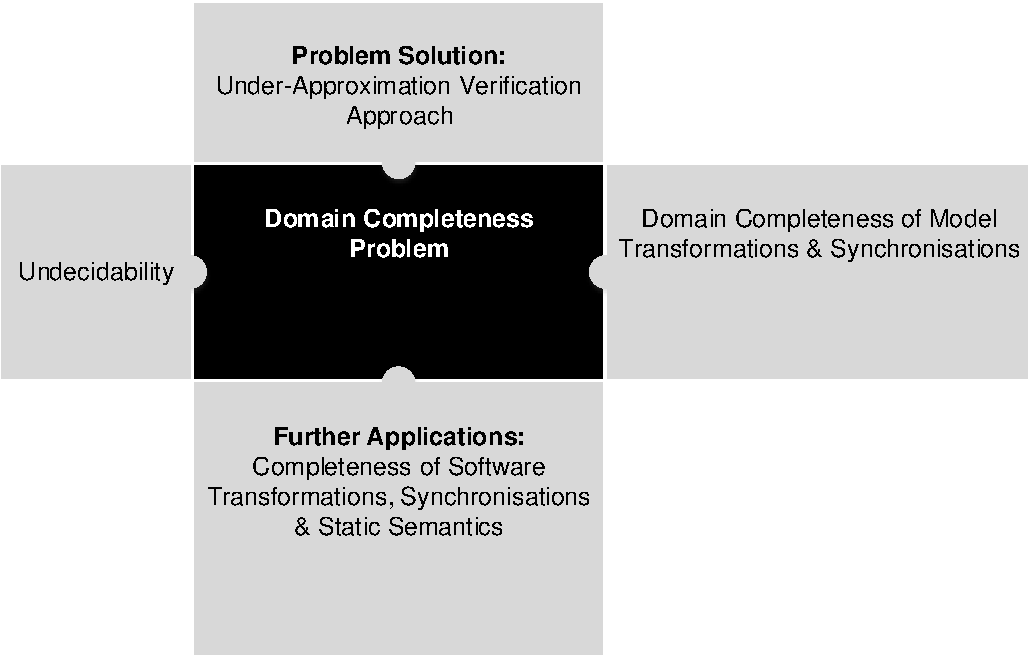
\includegraphics[width=.9\textwidth]{img/gen_intro/bigpicture.pdf}};
\fill (-1.5,.1) node[inner sep=1pt] (B) {\Large{\textcolor{white}{$\Lang(C) \subseteq \Lang(\GG)$?}}};
\fill (3.85,.1) node[inner sep=1pt] (C) {\Large{$\Lang(C) \subseteq \Lang(\TGG)^S$}};
\fill (-1.45,-3.4) node[inner sep=1pt] (D) {\Large{$\Lang(\EBNF) \equiv \Lang(C)$}};
\end{tikzpicture}
\end{center}
\caption{Main Results of this Thesis}
\label{fig:sec-gen-intro-org:bp}
\end{figure}

\cref{fig:sec-gen-intro-org:bp} presents the main results of this thesis.
The domain completeness problem is introduced as the core problem statement.
Generally, we assume that the set of allowed models (graphs) in a given domain of discourse $D$, i.e., the visual domain-specific modelling language (DSL) of $D$, is defined by a set of (domain) graph constraints.
A graph constraint formulates structural restrictions on graphs.
Given a set of constraints $C$, then $\Lang(C)$ is the set of all graphs that satisfy the restrictions which are formulated by the domain constraints in $C$.
Therefore, $\Lang(C)$ is the set of allowed models (graphs) in the given domain $D$, i.e., $\Lang(C)$ is the DSL of $D$.
On the other hand, a set of graph transformation rules together with a start graph form a graph grammar $\GG$.
With $\Lang(\GG)$ we denote the language of graphs that can be created by rule applications starting at the start graph.
The domain completeness problem is defined as follows: Does it hold that $\Lang(C) \subseteq \Lang(\GG)$?
Therefore, can all graphs that satisfy the domain constraints in $C$ be created from the start graph in $\GG$ by successively applying the rules of graph grammar $\GG$? - OR - Is the set of domain constraints $C$ as restrictive as or more restrictive than grammar $\GG$, respectively? - OR - Is DSL $\Lang(C)$ completely covered by the graph grammar $\GG$?

It turns out that the domain completeness problem is undecidable in general, i.e., we cannot find a complete computable solution to this problem.
Therefore, we propose an under-approximation solution to the domain completeness problem in order to verify the language inclusion $\Lang(C) \subseteq \Lang(\GG)$ of domain completeness approximately.
Basically, the solution consists of a set of conditions that are sufficient but not necessary and need to be verified.
Therefore, the solution may lead to false negatives but not to false positives, i.e., if the conditions are fulfilled, then it is ensured that the language inclusion holds. 
If the conditions are not fulfilled, then the language inclusion may hold or not hold and additional checks may be necessary in order to obtain (partial) truth.

Furthermore, we developed three main applications of the solution (cf. \cref{fig:sec-gen-intro-org:bp}).
%Initially, we stated the domain completeness problem in view of model transformations and generalised the problem to general graph grammars afterwards.
The domain completeness problem of model transformations is stated as follows: Can all allowed models in the given domain $D$ (all graphs in $\Lang(C)$) be transformed based on a given triple graph grammar $\TGG$? - OR - Does it hold that $\Lang(C) \subseteq \Lang(\TGG)^S$ for forward model transformations or $\Lang(C) \subseteq \Lang(\TGG)^T$ for backward model transformations?
%In order to return to the initial idea, 
Therefore, we have instantiated our solution to the approximate verification of the language inclusion $\Lang(C) \subseteq \Lang(\TGG)^S$ or $\Lang(C) \subseteq \Lang(\TGG)^T$, respectively.
Thus, the language inclusion problem is stated in the context of a triple graph grammar $\TGG$ \cite{DBLP:journals/eceasst/AnjorinLS15,DBLP:conf/gg/SchurrK08,DBLP:conf/wg/Schurr94} instead of a flat graph grammar $\GG$ where the $\TGG$ specifies the model transformation.
The domain completeness problem of model synchronisations is stated analogously: Can all allowed model updates in the given domain be synchronised?
We show that this problem can be verified based on the results of model transformations.
% According to \cref{sec-sem-cor}, the completeness results may ensure a complete validation of the semantic correctness of model transformations and synchronisations based on semantic checks.
The third application of the solution is to verify the completeness of software transformations and synchronisations: 
\begin{enumerate}
  \item Can all programs (their abstract syntax trees (ASTs)) written in a given programming language be transformed? 
  \item Can all program updates (updates of their abstract syntax trees (ASTs)) be synchronised?
\end{enumerate}
Programs written in a given programming language are represented by their abstract syntax models (ASTs) and transformed by performing model transformations of ASTs based on a given $\TGG$.
Commonly, programming languages are defined by a context-free word grammar.
Therefore the third application of the solution mainly focuses on %the 
solving the % Kommentar Frank
problem to close the gap between the word grammar world and graph world by presenting a mapping from a context-free grammar in Extended-Backus-Naur Form (EBNF) notation into a set of graph constaints $C$ such that the language of ASTs over the EBNF $\Lang(\EBNF)$ is equivalent (isomorphic) to $\Lang(C)$, i.e., $\Lang(\EBNF) \equiv \Lang(C)$.

\cref{fig:sec-gen-intro-org:publications} presents the peer-reviewed publications for the period of this thesis and their assignment to the corresponding chapters.
Publications that are not assigned to a chapter contain no direct contribution to this thesis.

\begin{figure}[!tb]
\begin{center}
\begin{tabular}{| p{6.5cm} | p{5.5cm} | c |}
  \hline			
  \textbf{Title} & \textbf{Authors} & \textbf{Chapter} \\
  \hline
  Towards the Propagation of Model Updates along different Views in Multi-View Models \cite{DBLP:conf/etaps/GottmannNE0E16} &
  Susann Gottmann, Nico Nachtigall, Claudia Ermel, Frank Hermann, Thomas Engel & 
  - \\
  \hline
  Triple Graph Grammars in the Large for Translating Satellite Procedures \cite{DBLP:conf/icmt/0001GNEBMPEE14} & 
  Frank Hermann, Susann Gottmann, Nico Nachtigall, Hartmut Ehrig, Benjamin Braatz, Gianluigi Morelli, Alain Pierre, Thomas Engel, Claudia Ermel & 
  \cref{sec-compl-software-trans} \\
  \hline
  Solving the FIXML2Code-case Study with HenshinTGG \cite{DBLP:conf/staf/0001NBEG14} & 
  Frank Hermann, Nico Nachtigall, Benjamin Braatz, Thomas Engel, Susann Gottmann & 
  - \\
  \hline
  Towards Domain Completeness for Model Transformations Based on Triple Graph Grammars \cite{DBLP:conf/staf/Nachtigall0BE14} & 
  Nico Nachtigall, Frank Hermann, Benjamin Braatz, Thomas Engel & 
  \cref{sec-dom-compl} \\
  \hline
  On an Automated Translation of Satellite Procedures Using Triple Graph Grammars \cite{DBLP:conf/icmt/HermannGNBMPE13} & 
  Frank Hermann, Susann Gottmann, Nico Nachtigall, Benjamin Braatz, Gianluigi Morelli, Alain Pierre, Thomas Engel & 
  \cref{sec-compl-software-trans} \\
  \hline
  Correctness and Completeness of Generalised Concurrent Model Synchronisation Based on Triple Graph Grammars \cite{DBLP:conf/models/Gottmann0NBEEE13} & 
  Susann Gottmann, Frank Hermann, Nico Nachtigall, Benjamin Braatz, Claudia Ermel, Hartmut Ehrig, Thomas Engel & 
  \cref{sec-dom-compl-synch} \\
  \hline
  Symbolic Execution of Satellite Control Procedures in Graph-Transformation-Based {EMF} Ecosystems \cite{DBLP:conf/models/NachtigallBE13} & 
  Nico Nachtigall, Benjamin Braatz, Thomas Engel & 
  \cref{sec-compl-oper-sem} \\
  \hline			
  Transformation Systems with Incremental Negative Application Conditions \cite{DBLP:conf/wadt/CorradiniHHGN12} & 
  Andrea Corradini, Reiko Heckel, Frank Hermann, Susann Gottmann, Nico Nachtigall & 
  - \\
  \hline  
\end{tabular}
\end{center}
\caption{List of Publications}
\label{fig:sec-gen-intro-org:publications}
\end{figure}

After we have introduced the main results, we refer briefly to their chapters.

\subsection{Chapter 2: Model Transformations, Model Synchronisations \& Formal Framework}
While \cref{sec-gen-intro} gives a general introduction to the topic, in \cref{sec-mt-ms-ff}, we give a more in-depth introduction to model transformations and synchronisations.
We recall different classes of transformations and synchronisations, i.e.:
\begin{enumerate}
  \item In-place transformations vs. ``external" transformations that preserve the source models,
  \item horizontal vs. vertical transformations,
  \item endogeneous vs. exogeneous transformations, and
  \item model (text)-to-model (text) transformations.
\end{enumerate}  
Moreover, we clarify how meta-modelling is linked to model transformations and synchronisations.

We recall basic definitions and results of the theory of algebraic graph transformation.
In particular this includes the category $\AGraphs_\ATGI$ of typed attributed graphs with node type inheritance, their rule-based transformation, graph grammars, (nested) graph conditions and constraints and $\M$-adhesive transformation systems that generalise the concepts from attributed graphs to a variety of different types of graphs (and other structures).
Note that the main results have been developed with a focus to be applied in $\AGraphs_\ATGI$.
Furthermore, we review the notions of triple graphs, triple graph grammars (TGGs) and model transformations / synchronisations based on TGGs.
Finally, we give an overview of important properties of model transformations and synchronisations with a focus to the completeness property.

\subsection{Chapter 3: Domain Completeness}
\cref{sec-dom-compl} introduces the domain completenes problem, shows its undecidability and presents an approximative solution to this problem.
It is shown how to verify the domain completeness problem.
Moreover, limitations of the verification approach are discussed and the concept of recursive graph constraints is introduced in order to allow an application of the approach in the context of infinite domain constraints.
For example, infinite graph constraints are used when describing regular paths in graphs. 
Two methods are presented for deriving finite graph constraints from infinite graph constraints such that the verification process can terminate.
Finally, we consider the verification of domain completeness under restrictions of the domain type graph.
This reflects the situation where only a subset of all constituents of the given domain is subjected to the verification.

\subsection{Chapter 4: Domain Completeness of Model Transformations \& Model Synchronisations}
In \cref{sec-dom-compl-mt-synch}, we instantiate the results from \cref{sec-dom-compl} to the verification of domain completeness of model transformations and model synchronisations.
We reformulate the completeness problem in the context of transformations and distinguish between forward and backward domain completeness of transformations and synchronisations.

\subsection{Chapter 5: Further Applications}
\cref{sec-further-appl} presents further applications of the previous verification results for domain completeness.
In particular, this includes the instantiation of the results to the verification of the completeness of software transformations and synchronisations.
Furthermore, it is shown to which extend the concept of recursive graph constraints from \cref{sec-dom-compl} can be used for the verification of completeness in the context of expressing static semantics in models.

\subsection{Chapter 6: Conclusion, Related \& Future Work}
In \cref{sec-conclusion} we conclude and discuss related work and aspects of future work.